
This chapter is about Partially Observable MDP (POMDP). The
main difference between MDP and POMDP is that in a POMDP we will not observe the current state but
only a signal that depends on it.


\paragraph{Example:}\ \\
Assume we have four states, in linear order: $1,2,3,4$. We have an
action UP that with probability $0.90$ moves from $i$ to $i-1$ and
with probability $0.1$ moves to $i+1$. Similarly, we have an action
DOWN that with probability $0.90$ moves from $i$ to $i+1$ and with
probability $0.1$ moves to $i-1$. (In state $i=1$ if we need to move
to $i-1$ we stay in $i=1$ and in state $i=4$ if we need to move to
$i+1$ we stays in state $i=4$.)

One of the states, state $2$ has a reward, while the other states do not have any reward. (See Figure~\ref{fig:Example-4states}.) The only observation we see is the reward.

Initially, we know we are in a random state without a reward. This implies that the state distribution of where we are is $(1/3,0,1/3,1/3)$.
Assume we did an action UP and did not observe a reward. We now can
compute the posterior of our probability distribution.

First, we compute the state probability distribution, given that we start at a given state and perform action UP.
\begin{enumerate}
\item
Assuming we are in state $i=1$, our state distribution will be
$(0.9,0.1,0,0)$.
\item
Assuming we are in state $i=2$, our state distribution will be
$(0.9,0,0.1,0)$.
\item
Assuming we are in state $i=3$, our state distribution will be
$(0,0.9,0,0.1)$.
\item
Assuming we are in state $i=4$, our state distribution will be
$(0,0,0.9,0.1)$.
\end{enumerate}

Since our prior state distribution was $(1/3,0/1/3,1/3)$ our
posterior state distribution (before observing the reward) is
$(0.3,1/3,0.3,1/15)$.

Given that we observed ``no reward'' we are not in state $2$ so the
posterior state distribution is $(0.45,0,0.45,0.1)$.

This example is an instance of a Bayesian computation. Namely, this example demonstrates how given a state distribution (often called ``prio''), and action we perform and an observation, we can compute the next state distribution. In the following we will generalize this example.

\begin{figure}
  % Requires \usepackage{graphicx}
  \begin{centering}
  
\includegraphics[width=0.1\textwidth]{figures/Example-4states.PNG}\\
  \caption{The four state POMDP}\label{fig:Example-4states}
  \end{centering}
\end{figure}


\section{POMDP: model}

The model of a POMDP will be similar to that of an MDP with an
additional observation function. Namely,
\begin{itemize}
\item
$S$, a finite set of states.
\item
$A$, a finite set of actions.
\item
$p(s'|s,a)$, a probability distribution of next state given that we
are in state $s$ and do action $a$.
\item
$R(s,a)$ a random variable for the reward in state $s$ doing action
$a$, and $r(s,a)=E[R(s,a)]$.
\item
$q_0$ the initial state (can also be a distribution over states)
\item
$Ob$ is an observability distribution over $O$ a set of observable
signals. $O$ can be either finite of infinite. $Ob(o|s',a)$ is the
probability that we observe signal $o\in O$ if we reach state $s'$
after doing action $a$. (Note that in an MDP we have the observable
signals $O=S$ and $Ob(o|s',a)=s'$.)
\end{itemize}

\subsection{Belief state}

The belief state tracks the state distribution, which captures our
current state. Each time we perform an action and observe an
observation we compute a new belief state, which is our posterior
distribution, given our action and observation.

The belief state is a sufficient statistics, implying that it has
all the information needed from the history. (Also, two histories which reach the same belief state, we should behave identically for them.)
%
Formally, a belief state $b$ is a distribution over states, i.e.,
$b\in[0,1]^{|S|}$ and $\sum_s b(s)=1$.

Given a belief state $b$ and an action $a$ and observation $o$, we
need to compute the next belief state $b'(s)=\Pr[s'|o,a,b]$. This
will be a deterministic function, and we will have $b'=T(b,a,o)$.

\paragraph{Belief state computation:}\ \\
We compute the next belief state as follows:
\begin{align*}
b'(s') &= \Pr[s'|o,a,b]\\
&= \frac{\Pr[o|s',a,b]\Pr[s'|a,b]}{\Pr[o|a,b]}\\
&= \frac{\Pr[o|s',a]\sum_s \Pr[s'|a,b,s]\Pr[s|a,b]}{\Pr[o|a,b]}\\
&= \frac{Ob(o|s',a)\sum_s p(s'|a,s)b(s)}{\Pr[o|a,b]}
\end{align*}
where the first identity is the definition of the new belief state.
The second identity is Bayes rule. The third identity is adding a
conditioning over $s$. The last identity is translating the
probabilities to the POMDP parameters.

The belief state is (almost) a linear operation, when we fix the action $a$ and the observation $o$.
We can define a matrix $M^{a,o}$, where $M^{a,o}[s',s]=Ob(o|s',a) p(s'|a,s)$, and we have $b'=M^{a,o}b/\Pr[o|a,b]$.

\paragraph{From POMDP to infinite MDP}\ \\
Consider the following MDP. The set of states are $B$, all the possible belief states. (Note that $B$ is infinite!) The set of actions is $A$ is the set set of action in the POMDP (finite). For each belief state $b$ and action $a$ we
define the expected reward $r(b,a)=\sum_s b(s)r(s,a)$. The
transition probability, given an action $a$ and an observation $o$,  is to move to $b':=T(b,a,o)$ and it is
deterministic. (Namely, $\Pr[b'=T(b,a,o)|b,a,o]=1$ and $\Pr[b'\neq
T(b,a,o)|b,a,o]=0$.)


\section{Value function}
The value function will be mapping belief states to expected return.
The return can be any of the return we discussed: finite horizon,
discounted, of average reward.

We would like to characterize the optimal value function. For a finite horizon it will be piece-wise linear and convex. (For discounted it will be convex.) Our algorithmic challenge is to handle the infinite space of belief states. We will concentrate on the case of finite horizon.

For simplicity, we start with a horizon of length $H=1$. Namely, we would like to maximize our immediate reward. For each action, our immediate reward is a linear function in the belief state. Namely, $r(b,a)=\sum_s b(s)r(s,a)$. The optimal action for $H=1$ is the action $a$ that maximizes the expected reward. Namely, $V^*_1(b)=\max_a r(b,a)=\max_a [\sum_s b(s)r(s,a)]$. This implies that the optimal value function is a maximum of linear functions, and hence convex. This also gives us a finite representations, since it also partitions the space of belief states to convex regions, and in each region there is an optimal action. The partition to the regions is done by intersecting hyper-planes. The region in which $a_1$ is the best action is define by $\{b: \forall a\neq a_1 \sum_s b(s)r(s,a_1)\geq \sum_s b(s)r(s,a)\}$.

We will now consider a horizon of $H=2$. We will partition the task to three steps. In the first step, we will assume that we are in belief state $b$ perform action $a_1$ and observe $o_1$. In the second step, we assume we are in belief state $b$ and perform action $a_1$. In the third step, we only assume we are in belief state $b$.

Assume we  we are in belief state $b$ perform action $a_1$ and observe $o_1$. We would like to compute $V_H(b|a_1,o_1)$ for $H=2$. For the first step, given that we do action $a_1$, we can compute the expected immediate reward $r(b,a_1)=\sum_s b(s)r(s,a_1)$. Now, we move from belief state $b$ to belief state $b'=T(b,a_1,o_1)$. When we reach $b'$ we have only one step remaining, so we perform the best action and get $V^*_1(b')$. This also implies that $V^*_2(b|a_1,o_1)=r(b,a_1)+V^*_1(b')$, where $b'=T(b,a_1,o_1)$. This implies that $V^*_2(b|a_1,o_1)$ is piece-wise linear.  (See Figure~\ref{fig:belief-state-1}.)

\begin{figure}
  % Requires \usepackage{graphicx}
  \begin{centering}
  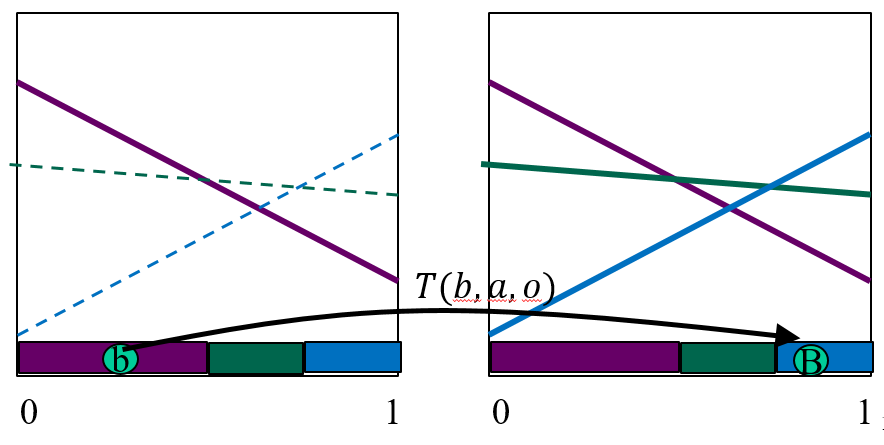
\includegraphics[width=0.5\textwidth]{figures/belief-state-1.PNG}\\
  \caption{Computing $V^*_2(b|a_1,o_1)$}\label{fig:belief-state-1}
  \end{centering}
\end{figure}

For the second step, we can now do the same for each possible observations (assume the set of observations is finite, for simplicity). This implies that we have the values of $V^*_2(b|a_1,o)$ for any $o\in O$. This allows us to compute $V^*_2(b|a_1)$, by simply averaging over the observations, i.e., $V^*_2(b|a_1)=\sum_o V^*_2(b|a_1,o)\Pr[o|b,a_1]$. We can compute $\Pr[o|b,a]=\sum_{s,s'} b(s)p(s'|s,a)Ob(o|s',a)$.

For the third step, given that we can compute $V_2^*(b|a)$ for any action $a\in A$, we
can deduce $V_2^*(b)=\max_a V_2^*(b|a)$.

We can now compute for a longer horizon, say $H=3$, using dynamic programming. We want to compute $V^*_3(b)$. We first compute the function $V_2^*(\cdot)$. For each action $a_i$ and observation $o_j$ we compute $V^*_3(b|a_i,o_j)$. This is done by first computing $r(b,a_i)$ and $b'=T(b,a_i,o_j)$. Then we compute $V^*_3(b|a_i,o_j)
= r(b,a_i)+V^*_2(b')$. By averaging over the observations $o_j$ we compute $V_3^*(b|a_i)=E_{o_j}[V^*_3(b|a_i,o_j)]$. By maximizing over the action $a_i$ we compute $V_3^*(b)=\max_{a_i} V^*_3(b|a_i)$

\paragraph{Optimal value function}\ \\
For the finite horizon the optimal value function $V^*_H(b)$ is
define as follows,
\[
V^*_H(b)=\max_a [r(b,a)+\sum_o \Pr[o|b,a]V^*_{H-1}(T(b,a,o))]
\]
and the optimal policy is
\[
\pi_H^*(b)=\arg\max_a [r(b,a)+\sum_o \Pr[o|b,a]V^*_{H-1}(T(b,a,o))]
\]

\begin{theorem}
\label{pomdp:thm:FH}
For the finite horizon, the function $V^*_H$ is piece-wise linear
and convex. In addition, there exists a collection of
$\Theta=\{\theta_i\in \mathbb{R}^{|S|}\}$ such that
$V^*_H(b)=\max_{\theta_i\in\Theta} \sum_s b(s)\theta_i(s)$.
\end{theorem}

For the discounted setting we have
\[
V^*(b)=[r(b,a)+\gamma\sum_o \Pr[o|b,a]V^*_{H-1}(T(b,a,o))]
\]
\begin{theorem}
For the discounted return, the function $V^*$ is convex.
\end{theorem}



\subsection{Value Iteration:}

We can run a value iteration in the POMDP (actually, on the belief states). We can write the update as follows:
\begin{align*}
V^{a,o}_{t+1}(b)=&\frac{r(b,a)}{|O|}+ \Pr[o|b,a]  V_t^*(T(b,a,o))\\
V_{t+1}^a(b)=&\sum_o V^{a,o}_{t}(b)= r(b,a)+ E_o [V_t^*(T(b,a,o))]\\
V_{t+1}^*(b)=&\max_a V_{t+1}^a(b) = \max_a [r(b,a)+\sum_o V_t^*(T(b,a,o))]
\end{align*}
%\begin{align*}
%V_{t+1}^*(b) =& \max_a [r(b,a)+\gamma\sum_o V_t^*(T(b,a,o)\\
%V_{t+1}^*(b)=&\max_a V_{t}^a(b)\\
%V_{t}^a(b)=&\sum_o V^{a,o}_{t}(b)\\
%V^{a,o}_{t}(b)=&\frac{r(b,a)}{|O|}+\gamma\Pr[o|b,a]V_t(T(b,a,o))
%\end{align*}

We can now prove Theorem~\ref{pomdp:thm:FH} by induction on $t$. The base of the induction is $t=1$. For $\Theta_1=\{r(\cdot,a)\}$ we have that $V^*_1(b)=\max_{\theta\in\Theta_1}b^\top \theta$.

For the induction step, assume that $V_t^*$ is a maximum of linear functions. Namely, there exists a set $\Theta_t$ such that
\[
V^*_t(b)=\max_{\theta\in\Theta_t}\theta^\top b
\]
For $V_{t+1}^{a,o}$ we have that $b'=T(b,a,o)$ is linear in $b$, i.e., there is a matrix $M^{a,o}$ such that $b'=M^{a,o}b/\Pr[o|b,a]$. (Note that $M^{a,o}$ depends on
$a$ and $o$.) The value of $V_t^{a,o}$ is
\begin{align*}
V_{t+1}^{a,o}(b)
&=\frac{r(b,a)}{|O|}+ \Pr[o|b,a]  V_t^*(b')\\
&= \frac{r(\cdot,a)^\top b}{|O|}+  \Pr[o|b,a]  \max_{\theta\in\Theta_t} \theta^\top b'\\
&= \frac{r(\cdot,a)^\top b}{|O|}+  \max_{\theta\in\Theta_t} \theta^\top M^{a,o}b
%\end{align*}
\end{align*}

This implies that we can define $\Theta_{t+1}^{a,o}=\{\frac{r(\cdot,a)^\top}{|O|}+\theta^\top M^{a,o}:\theta \in \Theta_t\}$ and have
\[
V_{t+1}^{a,o}(b)= \max_{\theta\in\Theta_{t+1}^{a,o}}  \theta^\top b
\]

For $V^a_{t+1}$ we have that
\[
V_{t+1}^a(b)=\sum_o V_{t+1}^{a,o}(b)=\sum_o \max_{\theta\in\Theta_{t+1}^{a,o}}
\theta^\top b=\max_{\theta\in\Theta_{t+1}^{a}}\sum_o  \theta^\top b
\]
where
\[
\Theta^a_{t+1}=\{\sum_o
\theta^{a,o}|\theta^{a,o}\in\Theta^{a,o}_t\}
\]

For $V_{t+1}^*$ we have
\[
V^*_{t+1}(b)=\max_a V_t^a(b)=\max_{\theta\in\Theta_{t+1}}
\theta^\top b
\]
where $\Theta_{t+1}=\cup_a \Theta^a_t$.
%
This shows that the optimal value function $V^*$ is piece-wise linear, and is the maximum of linear functions.

The complexity of value iteration depends on the size of $\Theta_{t+1}$. For each action $a$ and observation $o$ we have $|\Theta^{a,o}_{t+1}|\leq |\Theta_t|$. For each action $a$ we have $|\Theta^a_t|\leq {|\Theta^{a,o}_{t+1}|}^{|O|}\leq {|\Theta_t|}^{|O|}$. For $\Theta_{t+1}$ we have $|\Theta_{t+1}|\leq \sum_a |\Theta_t^a|\leq |A|\cdot |\Theta_t|^{|O|}$.
This implies that $|\Theta_H|\leq |A|^{|O|^H}|\Theta_1|^{|O|^H} \leq |A|^{2|O|^H}$, since $|\Theta_1|\leq |A|$.

The above shows that while we can have a very interesting characterization for the optimal value function, a straightforward computation will be very inefficient, even for small number of actions and observations.  

%The complexity grows exponentially in $|O|$ with each iteration!

%Practical algorithms try to use pruning to reduce the size of $\Theta_t$, but the exponential time seems unavoidable.

%Pruning can help, but the exponential time seems unavoidable.

\subsection{Hardness}

Many computational problems related to POMDPs are hard. For the finite horizon, even with a unique start state, it is P-SPACE complete to compute the return of the optimal policy. For the finite horizon, in the case that there are no observations, it is NP complete to compute the return of the optimal policy. We
will show this simple hardness result in the following.

Assume we have no observations. This implies a policy simply selects a sequence of $H$ actions. The optimal policy will be the sequence of $H$ actions that will maximize the return. We will show a reduction to SAT.

Given a SAT formula over $n$ variables we create the following POMDP. For each clause we create the following POMDP gadget. We have two actions $0$ and $1$. We create two lines of length $n$, one line ends in a state with reward $1$ and the other in a state with reward $0$. All other rewards will be zero. We ``think'' of the state in the line as a number in $[1,n]$ and we associate the state $i$ it with the variable $x_i$. (See the lecture slides)

We start at the line ending with $0$. All the transition of states in the line ending in $1$ simply continue to the next state, i.e., from $i$ to $i+1$ (for both actions). For the line ending in zero, for each state $i$ where $x_i$ nor $\bar{x}_i$ do not appear in the clause, we continue to the next state on this line, with both actions.

For state $i$ in the line that ends in $0$, if $x_i$ appears in the clause, then in state $s_i$ with action $1$ we move to the $i+1$ state in the line ending in $1$, and with action $0$ we move to state $i+1$ in the line ending in zero. Similarly, if $\bar{x}_i$ appears in the clause,  then in state $s_i$ with action $0$ we move to the $i+1$ state in the line ending in $1$, and with action $1$ we move to state $i+1$ in the line ending in zero.

In the gadget, a sequence of $n$ actions will lead to the reward $1$ if and only if it represents an satisfying assignment to the clause.

We now take the gadgets for all the clauses, and select our initial state to uniformly at random to be the start state of one of the gadget (which represent a clause).

If the SAT formula is satisfiable, there is an assignment that satisfies all the clauses. Therefore guarantees a return of $1$.

Otherwise for each sequence of action, which represent an assignment, there is some clause which is not satisfied This implies that the return is at most $1-1/m$, where $m$ is the number of clause.

\paragraph{Remark:} Actually, we can get from the same reduction also a hardness to approximate result. We simply consider the MAX-SAT problem. For 3-SAT it is NP-hard to decide distinguish between satisfying $7/8+\epsilon$ of the terms or all the terms. This implies that it is NP-hard to distinguish between a return of $7/8+\epsilon$ or $1$.

\subsection{Policy Tree}

How does the optimal finite horizon policy can be implemented. Alternatively, how can we specify a general policy in a POMDP with a finite horizon. A policy tree is one simple approach to define a policy.

A policy tree is define using a tree. Each node of the tree, is label it an action, this will be the action we preform when we reach that node. The outgoing edges of each node are labeled by the observation. The depth of the tree, for a finite horizon return, is the length of the horizon.

We use the policy tree in the following way. Initially, we start at the root of the tree. The action which labels the root is the action we perform at the initial state. Given the observation we receive, we continue to the next node in the tree, following the edge labeled by this observation. We reach a new node. The label of that node is the action we perform and so on. Since the depth of the tree is the horizon $H$ for a finite horizon return, we can specify all the required actions. Note that each tree node is visited at most once during an episode.

The policy tree can be used to encode any history dependent  policy for the finite horizon return. The path from the root to a node encodes the history, when we consider both the node labels and the edge labels. Given the history we can encode in the next tree state the action of the policy given that history. 

\subsection{Automata Policy}

Another simple class to describe the policy is a finite automata with output, which is called a Moore automata. The outputs will be the selected actions and the inputs are the observations. While it is true that this class of policies is not universal, namely, not any policy can be represented in this way, many policies can be represented. Unlike the policy tree, this class can be used also for average reward and discounted return, since we can revisit nodes.

An important observation regarding this class of polices is that we can efficiently compute the value function of a given automata policy. Assume that $\pi$ is described by an automata policy. The expected discounted return of $\pi$ from
state $s$ when its automata is in state $\sigma$ and the last observation was $o$ is
\[
V^\pi(s;\sigma,o)=r(s,a)+\gamma \sum_{o',s'}
p(s'|s,a)Ob(o'|s'a)V^\pi(s';\sigma',o')
\]
where $a=\pi(\sigma,o)$ the action selected by $\pi$ when in state $\sigma$ of the automata and observes $o$, and $\sigma'$ is the next state in the automata, given we are in state $\sigma$ and observe $o$.

This implies that we have a set of linear equations and we can solve them efficiently. Note that the expected value of a policy $\pi$ is $V^\pi(s_0;\sigma_0,o_0)$, which is the expected return when the POMDP starts at node $s_0$, and the policy automata at $\sigma_0$ with observation $o_0$.


\section{Reusable trajectories}

Our goal is given a set of deterministic policies $\Pi$, to estimate
for each $\pi\in \Pi$ the value $V^\pi(s_0)$, its expected return.
We want a set of trajectories that would be relatively small
compared to $\Pi$, hopefully logarithmic in $|\Pi|$.

We will generate a set of trajectories $\Gamma$ in the following
simple way. We use a completely random policy to select the actions.
Namely, $\pi_R(a|b)=1/|A|$. We generate $m$ such trajectories.

We estimate the return of a policy $\pi\in \Pi$ in the following way. Let $\Gamma_\pi$ all the trajectories that agree with $\pi$. Formally, a deterministic policy $\pi$ accepts a trajectory $h=(s_0,a_0,o_0, \ldots s_H)$ if for every time $t$ we have that $a_t=\pi(h_{t-1})$ where $h_{t-1}$ is the history $h$ until time $t-1$.
%(Recall, $\pi$ is deterministic.) 
We set
\[
\hat{V}^\pi(s_0)=\frac{1}{|\Gamma_\pi|}\sum_{h\in \Gamma_\pi}
return(h)
\]

The main issue will be: how large $m$ has to be, in order to
guarantee with probability $1-\delta$ that the error for any $\pi\in
\Pi$ in the estimation will be at most $\epsilon$. We will look at
$m$ as a function of the error $\epsilon$, the confidence $\delta$,
the number of policies $|\Pi|$, and the maximum return $V_{max}$.

The proof follows in the following steps. Let $acc_\pi(h)=1$ if
$\pi$ agrees on all the actions in $h$. The following lemma states
that for any policy, the probability that it agrees with the
trajectory of length $H$ is exactly $1/|A|^H$.
\begin{lemma}
For a finite horizon $H$, for any policy $\pi$ we have
$\Pr_h[acc_\pi(h)=1]=\frac{1}{|A|^H}$.
\end{lemma}

Let $D_\pi$ be the distribution over histories generated by policy
$\pi$. The following lemma states that the distribution of the
random policy, condition of policy $\pi$ agreeing with the actions,
is identical to that of generated by policy $\pi$.
\begin{lemma}
\[
D_\pi(h)=D_{\pi_R}(h|acc_\pi(h)=1)
\]
\end{lemma}

The following lemma states that with high probability, for every
$\pi\in \Pi$ we have that the size of $|\Gamma_\pi|$ is exponential lower bounded as follows.
%in the horizon.
\begin{lemma}
For
\[
m> 8|A|^{H}\frac{V^2_{max}}{\epsilon^2}\log(2|\Pi|/\delta)
\]
with probability $1-\delta/2$ for every $\pi\in \Pi$ we have
\[
|\Gamma_\pi|\geq \frac{m}{|A|^{H+1}}>
4\frac{V^2_{max}}{\epsilon^2}\log(2|\Pi|/\delta)
\]
\end{lemma}

The following lemma states that if every $\Gamma_\pi$ is of
sufficient size, then for each policy $\pi$ we have a good
approximation.
\begin{lemma}
If for every $\pi\in \Pi$ we have
\[
|\Gamma_\pi|\geq \frac{m}{2|A|^{H}}> 4
\frac{V^2_{max}}{\epsilon^2}\log(2|\Pi|/\delta)
\]
then with probability $1-\delta/2$, for every $\pi\in \Pi$ we have
\[
|\hat{V}^\pi (s_0)-V^\pi(s_0)|\leq \epsilon
\]
\end{lemma}


The theorem concludes and establishes the sample size for a PAC
guarantee.
\begin{theorem}
For
\[
m> 8|A|^{H}\frac{V^2_{max}}{\epsilon^2}\log(2|\Pi|/\delta)
\]
with probability $1-\delta$, for every $\pi\in \Pi$ we have
\[
|\hat{V}^\pi (s_0)-V^\pi(s_0)|\leq \epsilon
\]
\end{theorem}



















%
